
\section{Recursive Algorithms}

\key{recursion traces}{linear recursion}{binary recursion}{tail
recursion}{recursion trees}{incremental algorithms}{divide-and-conquer
algorithms}{merge-sort}

\defn{Recursive Function}{is a function which refers to itself in its
definition}

\par{A classical example of a recursive faction is the factorial function, which
calls itself always with an argument decreased by one in each call, until the
\ita{base case} 1 is reached.}
\par{All recursive definitions share these 2 properties, i.e they all have a
base case which tells us when to stop calling, and they must reduce the size of
the data set with each call}

\subsection{Recursion Trace}

\par{A recursion trace allows us to visually trace the execution of recursive
algorithms. We draw a box for each call with an arrow pointing downwards
connected to the next call, and an arrow pointing upwards with the returning
value of that call}

\ex{\vphantom{.\\}
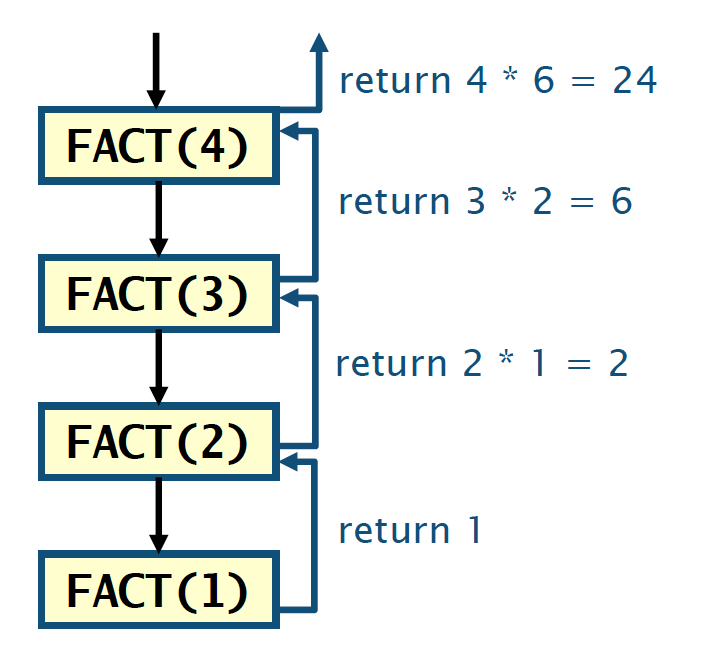
\includegraphics[width=0.4\textwidth]{fact}
}

\subsection{Linear Recursion}

\defn{Linear Recursion}{at most one recursive call with each iteration}

\rem{The space required to keep track of the recursive stack grows linearly with
$n$}

\rem{Useful when we view a problem in terms of a first/last element plus the
remaining set with the same structure (e.g sum array in haskell : \texttt{sum(l) =
head(l) + sum(tail(l))})}

\subsection{Tail Recursion}

\par{Though useful for designing short and elegant algorithms, recursive can
have a high memory cost, since the state of each recursive call must be stored
prior to being returned. This costs can sometimes be diminished by using a
recursive operation and the very last of the algorithm}

\defn{Tail Recursion}{is linear and the recursive call is its very last
operation}

\par{In tail recursive implementations, some variable is modified with each
call. There's no need to wait until the last call, since the updated variable is
immediately passed to the next recursive call. Hence, the state is passed onto
the call chain instead of being saved in memory}

\subsubsection{Recursive $\leftrightarrow$ Iterative}

\par{A common idiom is converting to/from tail recursive to iterative
algorithms. This is achieved by iterating through recursive calls, rather than
calling them explicitily}


\ex{~\cite{hochsteinSO}
\textbf{Recursive}
  \lstinputlisting[firstline=0, lastline=15]{recursionCode.js}
\textbf{Tail Recursive}
  \lstinputlisting[firstline=16, lastline=30]{recursionCode.js} 
\textbf{Iterative}
	\lstinputlisting[firstline=34, lastline=38]{recursionCode.js}
}

\subsection{Binary Recursion}

\defn{Binary Recursion}{when an algorithm makes two recursive calls}

\ex{Fibonacci : FIB(n-1) + FIB(n-2)}

\rem{Highly inefficient. Note how the same computations are made several times
over, in different calls. In the recursion tree there are $O(2^n)$ recursive
calls, i.e exponential complexity~\mymarginpar{recall memoization technique from
1P}}

\section{Algorithm Design Paradigms}

\subsection{Incremental}

\par{The solution of a problem is built one element at a time}

\ex{\vphantom{.\\}
\par{Sort sub array ; pick unvisited node ; add to sorted subarray}

\lstinputlisting[firstline=0, lastline=8]{algCode.py}
}

\subsection{Divide-and-Conquer} 

\par{Recursive algorithm, with 3 steps}

\begin{enumerate}
	\item Divide into smaller subproblems equivalent to the original 
	\item Conquer by solving subproblems recursively
	\item Combine the solutions to the subproblems to give the general solution
\end{enumerate}

\ex{\vphantom{.\\}

\par{\textbf{Merge-Sort} (1) split the array into two subarrays of size
$\frac{n}{2}$ ; (2) scan two smaller arrays simultaneously ; (3) add minimum to
sorted array, incrementing the pointer of the array from where the value was
removed; when fully scanned copy the remaining sub array to main array}
}

 
